\section{Results for two-dimensional discs}
We first present results from FARGO simulations. The 2D disc spans
$[R_\mathrm{min}, R_\mathrm{max}] = [0.4,10]R_0$. This gives a total
disc mass $M_{d}=0.086M_*$. The mass within
$R\in[R_\mathrm{min},R_{d1}]$ is $0.017M_*$, that within
$R\in[R_{d1},R_{d2}]$ is $0.049M_*$, and that within
$R\in[R_{d2},R_\mathrm{max}]$ is $0.021M_*$. We use a resolution of
$N_R\times N_\phi = 1024\times 2048$, or about $16$ grids per $H$, and
adopt $\epsilon_g=10^{-4}H$ for the   
self-gravity softening length\footnote{In 2D self-gravity, $\epsilon_g$ also
  approximates for the vertical disc thickness, so a more appropriate
  value would be $\epsilon_g\sim H$ \citep{muller12}. However, because
  $\epsilon_g\propto R$ is needed in FARGO, the Poisson kernel
  (Eq. \ref{2d_grav}) is no longer symmetric in $(R,R^\prime)$. We
  choose a small  
  $\epsilon_g$ in favour of angular momentum conservation, keeping in
  mind that the strength of self-gravity will be over-estimated.}.


\subsection{Reference run with random perturbations}
In this fiducial simulation we subject the disc to initial perturbations in
cylindrical radial velocity, 
\begin{align}\label{randpert}
  \frac{\delta v_R}{c_s} = \frac{\delta}{M}\times T(R) \sum_{m=1}^M\cos{m\phi},
\end{align}
where $\delta$ is an amplitude and 
\begin{align}
  T(R) =
  \exp{\left[-\frac{1}{2}\left(\frac{R-\overline{R}_d}{\Delta
          R_d}\right)^2\right]}, 
\end{align}
where $\overline{R}_d = (R_{d1}+R_{d2})/2$ and $\Delta R_d =
(R_{d2}-R_{d1})/2$. We use $M=10$ and choose
$\delta\in[-10^{-3},10^{-3}]$ randomly but independent of $\phi$. 

Fig. \ref{fargo_modeamp} plots evolution of the maximum
non-axisymmetric surface density amplitudes in $R\in[R_{d1},R_{d2}]$
for $m\in[1,10]$. Snapshots from the simulation are shown in
Fig. \ref{fargo_2d}. 
At early times $t\lesssim100P_0$ the dead zone is
dominated by low-amplitude high-$m$ perturbations. The $m\geq4$ modes
growth initially and saturate (or decays) after $t=40P_0$. Notice the
low $m\leq 2$ modes decay initially, but grows between $t\in[20,40]P_0$,
possibily due to saturation of the high-$m$ modes  
\citep{laughlin96,laughlin97}. However, the $m=1$ mode begins to grow
again after $t=70P_0$, and eventually dominates the dead zone. 

\begin{figure}
  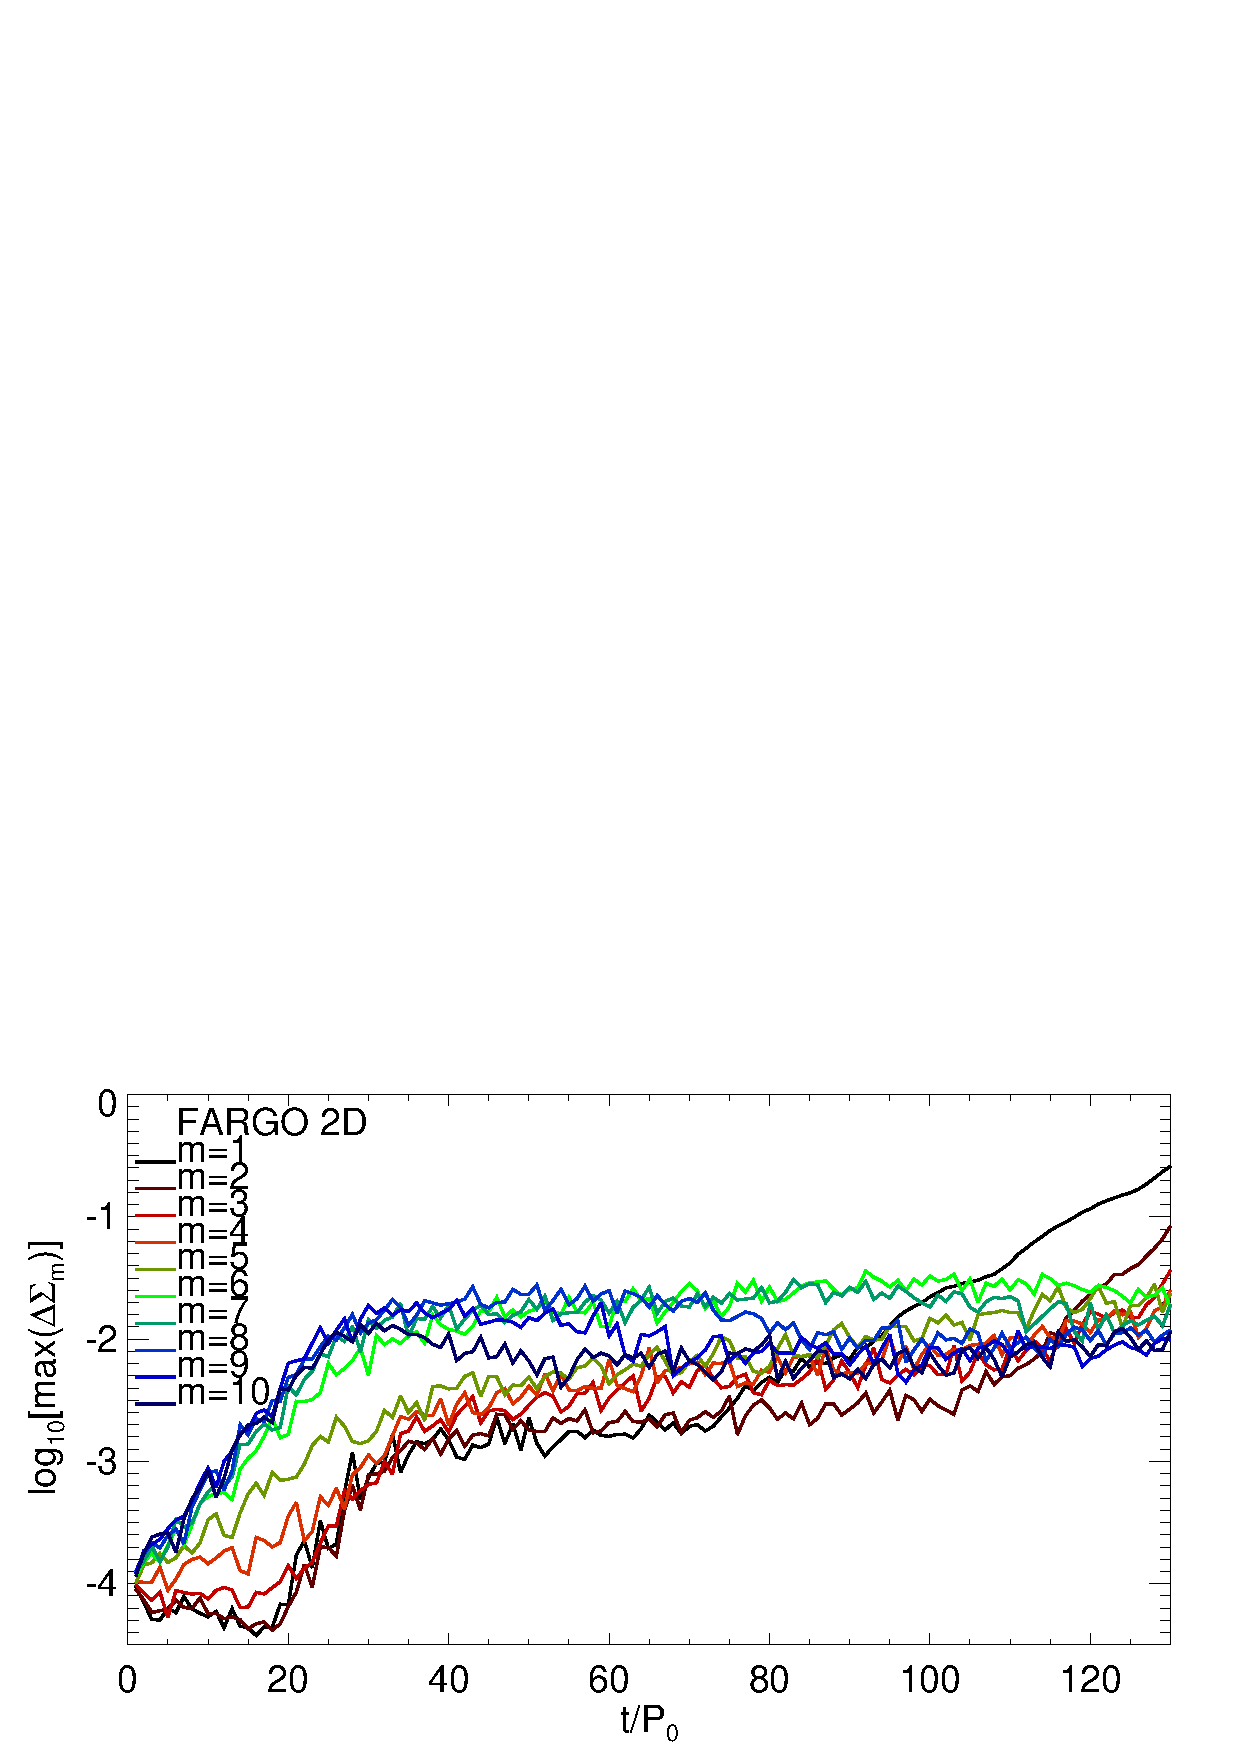
\includegraphics[width=\linewidth]{figures/nonaxi_evol_DZ_fargo}
  \caption{Evolution of maxima in non-axisymmetric surface density 
    in the fiducial FARGO simulation.\label{fargo_modeamp}} 
\end{figure}

\begin{figure}
  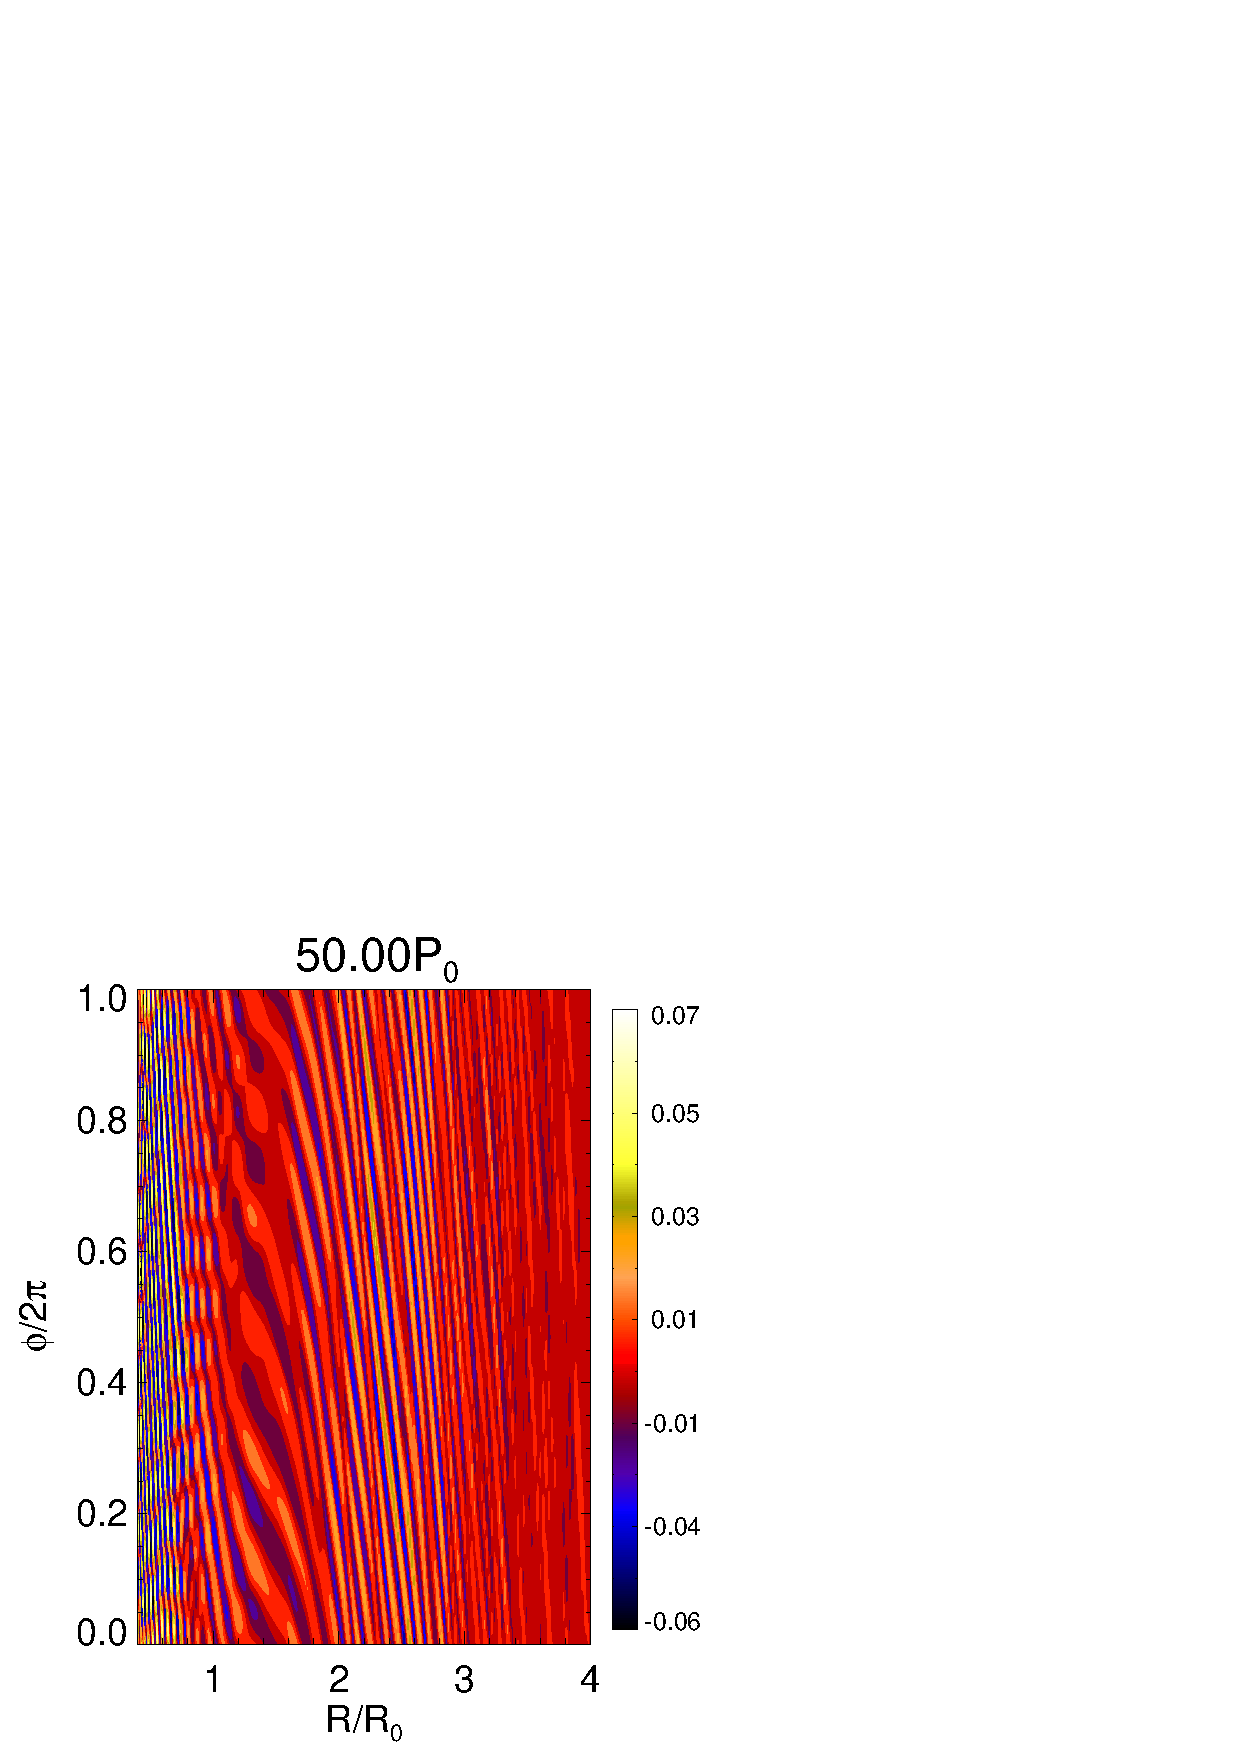
\includegraphics[scale=0.27]{figures/polarxy_dens050}\includegraphics[scale=0.27,clip=true,trim=2.26cm
  0cm 0cm
  0cm]{figures/polarxy_dens110}\includegraphics[scale=0.27,clip=true,trim=2.26cm
  0cm 0cm 0cm]{figures/polarxy_dens130} 
  \caption{Visualisation of the FARGO 2D simulation. The total  
    non-axisymmetric surface density
    $\Delta\Sigma$ is shown. \label{fargo_2d}} 
\end{figure}

Fig. \ref{2d_angmom} shows the disc angular momenta
evolution. Only the $m=0,\,1$ components are 
plotted since they are dominant. The $m=1$ structure has
an associated negative angular momentum.   
Its growth is compensated by an increase in the axisymmetric
component of angular momentum, such that $\Delta J_0 + \Delta
J_1 \sim 0$. Note that FARGO does not conserve angular momentum
exactly. However, we find the total angular momentum varies by 
$|\Delta J/J|= O(10^{-6})$, and is much smaller in magnitude than the
change in the angular momenta components, $|\Delta J_{0,1}/J|>
O(10^{-5})$. Fig. \ref{2d_angmom} then suggest that angular momentum
is transferred from the one-arm spiral to the background disc.    

\begin{figure}
  % scale=0.41
  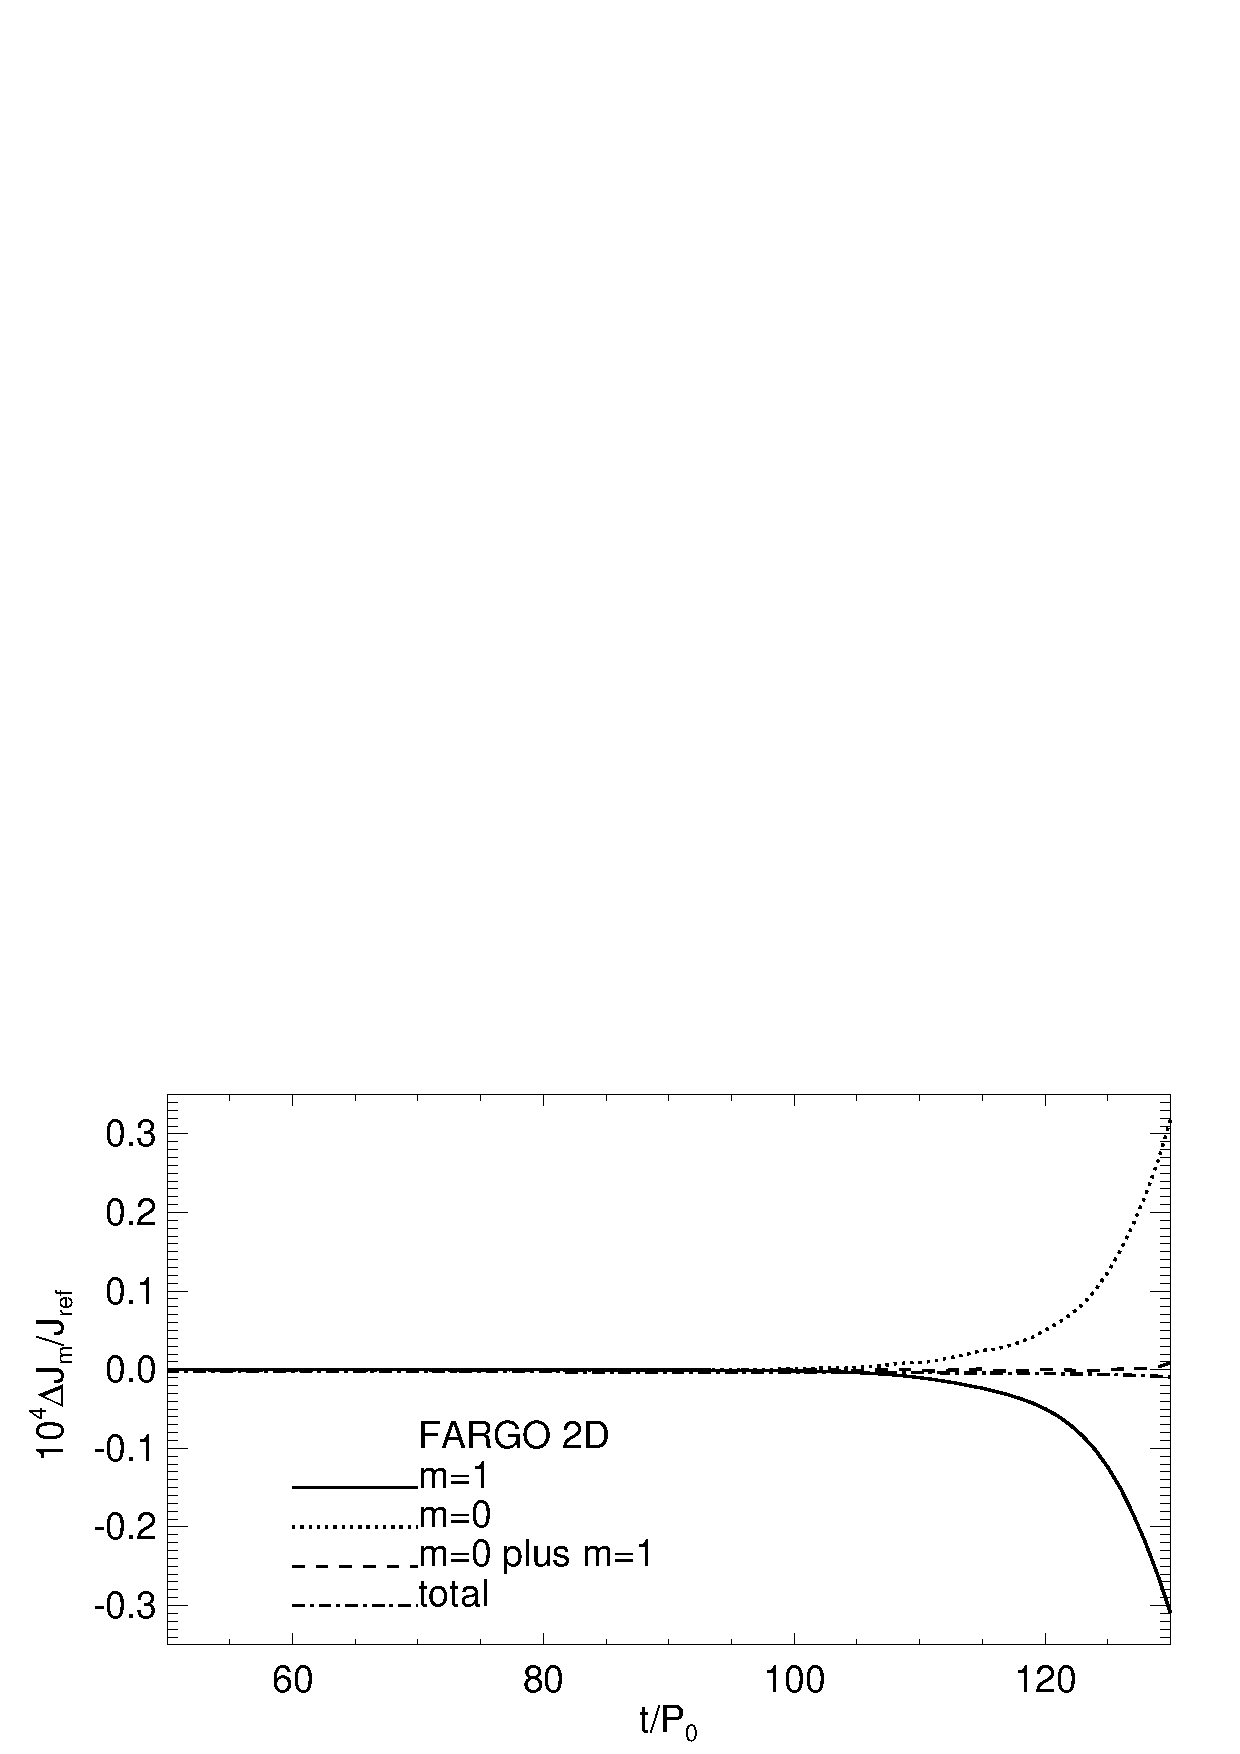
\includegraphics[width=\linewidth]{figures/nonaxi_evol_ang_fargo}
  \caption{Evolution of angular momentum components in the fiducial
    FARGO simulation. The perturbation
    relative to $t=0$ in 2D is shown in units of the
    initial total angular momentum $J_\mathrm{ref}$.\label{2d_angmom}} 
\end{figure}   

\subsection{Non-linear initial perturbation}\label{fargo_nonlin}
In order to focus on the one-arm spiral that emerges in the above
simulation, we here analyse a run with only an initial $m=1$
perturbation in the dead zone. Specifically, we set
\begin{align}
  &\Sigma \to \Sigma_0(R) + \delta\Sigma_0(R) + 2\Sigma_1(R)\cos{\phi},\\
  &v_\phi  \to v_{\phi 0}(R) + 2v_{\phi 1}(R)\cos{\phi},
\end{align}
for $R\in[R_{d1},R_{d2}]$, where
\begin{align}
  &\delta\Sigma_0 =
  -\delta^2\times\Sigma_0(R_{d1})\frac{R_{d1}}{R}\sin^3{\left[\frac{2\pi\left(R-R_{d1}\right)}{R_{d2}-R_{d1}}\right]},\\ 
  &\Sigma_1 =
  \delta\times\Sigma_0\sin{\left[\frac{\pi\left(R-R_{d1}\right)}{R_{d2}-R_{d1}}\right]},  
\end{align}
with $\delta = 10^{-3}$, and
\begin{align}
  v_{\phi 1} = -\frac{v_{\phi 0}\delta\Sigma_0}{2\Sigma_1}. 
\end{align}
This perturbs the dead zone structure while conserving total mass and
angular momentum. The $m=1$ perturbation has an associated negative
angular momentum (as observed in the previous simulation) at the
expense of increasing the angular momentum associated with the
background disc. %local exchange for simplicity 
%actually doesn't matter if we set plus or minus
Note that the perturbation to the axisymmetric surface density is
$O(\delta^2)$, whereas that in $m=1$ is $O(\delta)$. Since $Q>1$
everywhere in the disc, there is no risk of axisymmetric gravitational
instability. 

While the above form of initial perturbations is artificial, we find 
the spiral that forms have similar properties (see below) to that found in the
previous simulation. However, the above perturbations have the
advantage of producing cleaner results without complications from
higher $m$ modes, and the required simulation time for the one-arm
spiral to emerge is significantly reduced. 

Fig. shows the evolution of angular momenta. 


\begin{figure*}
  % scale=0.41
  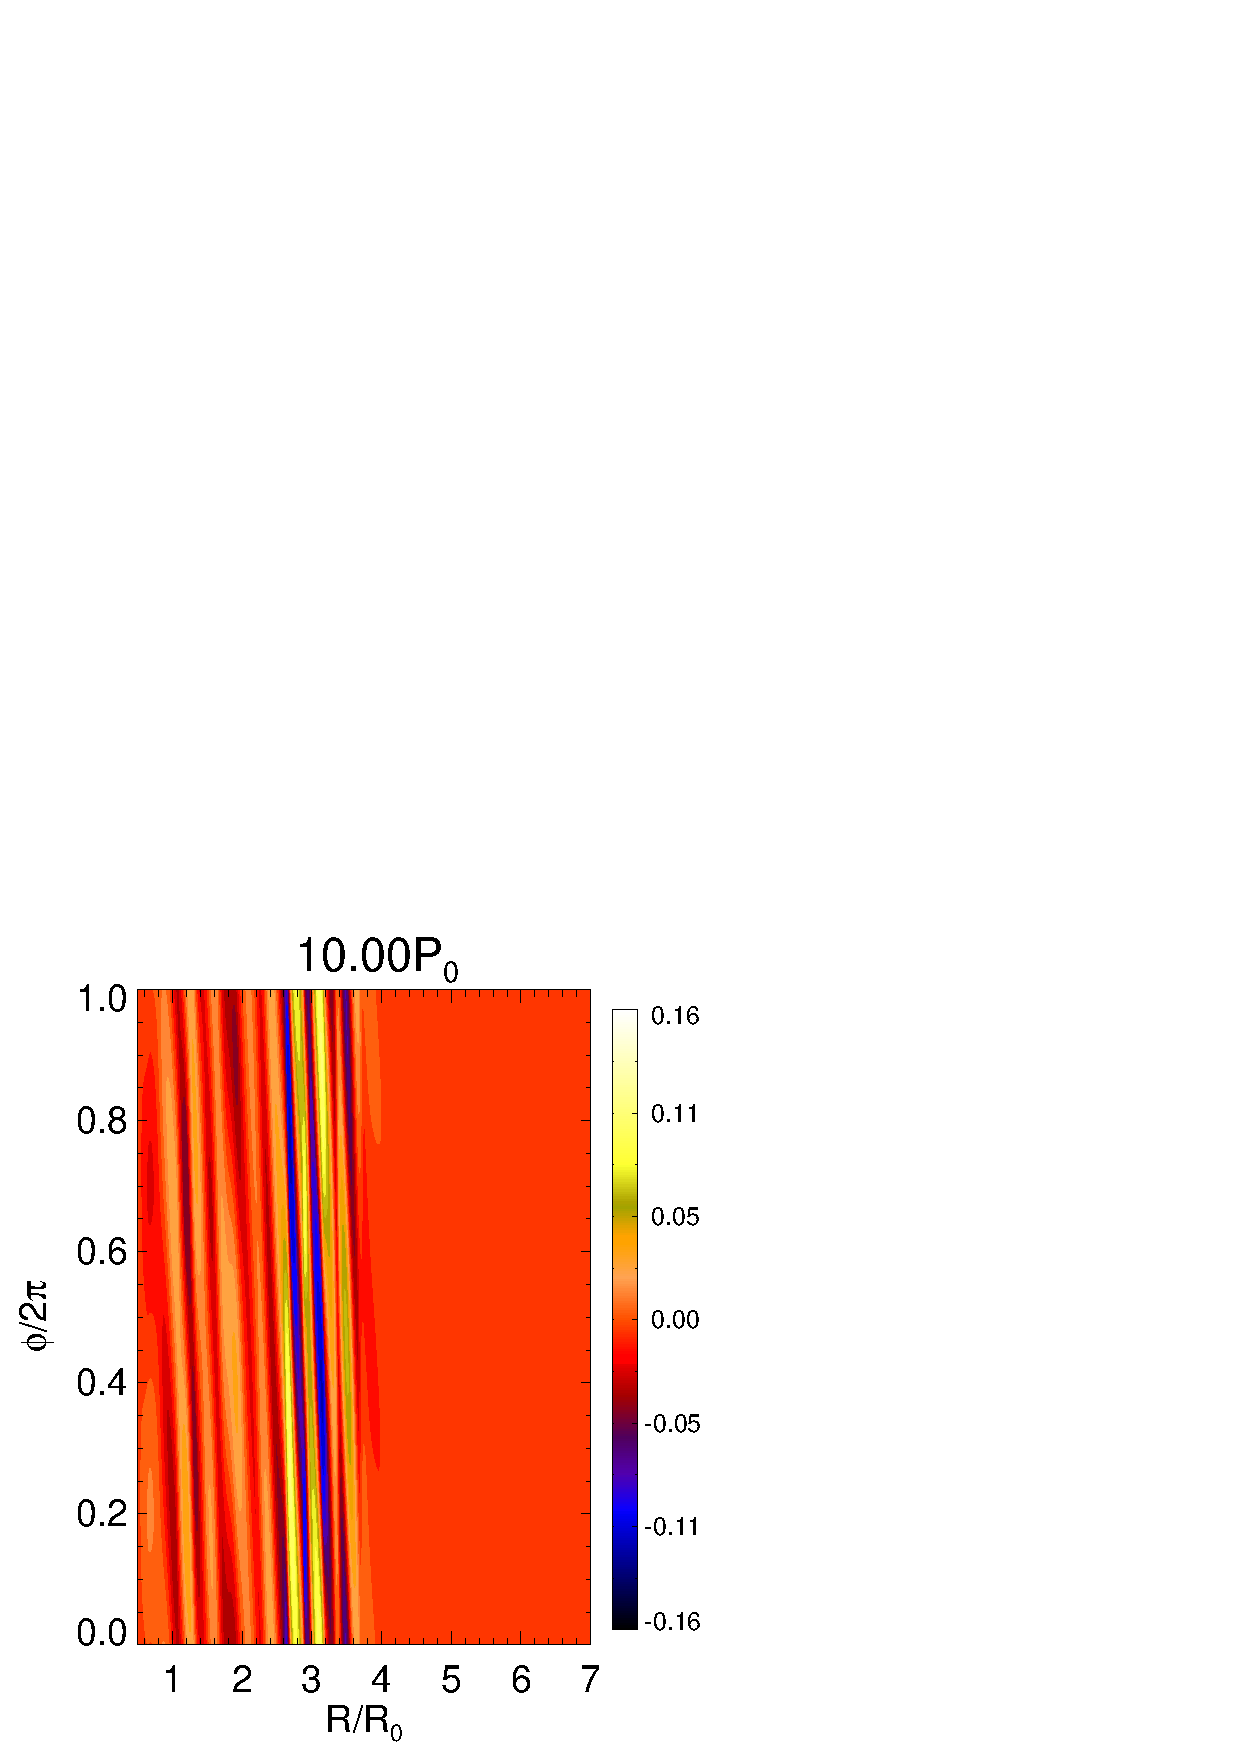
\includegraphics[scale=0.4,clip=true,trim=0cm 0cm 1.73cm
  0cm]{figures/polarxy_fargo_ex_100}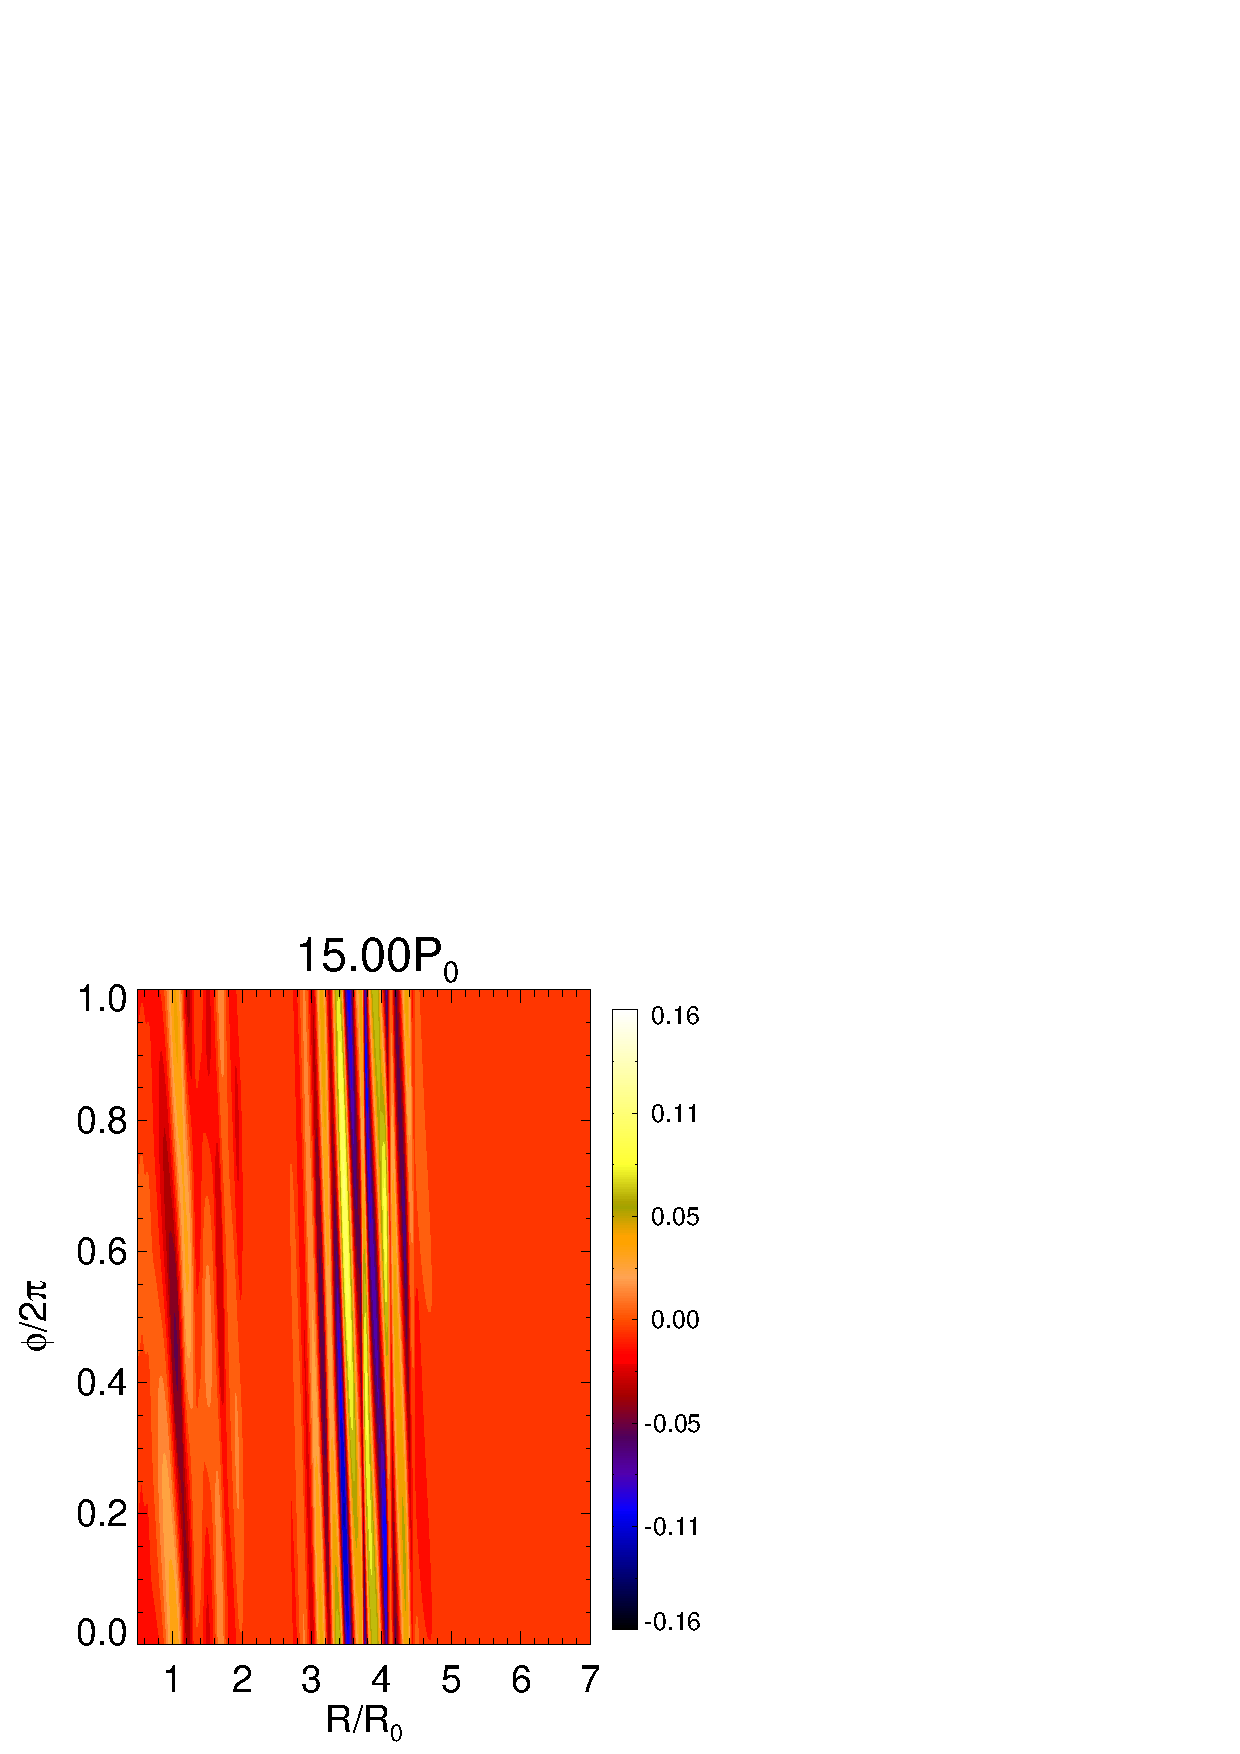
\includegraphics[scale=0.4,clip=true,trim=2.24cm
  0cm 1.73cm 0cm]{figures/polarxy_fargo_ex_150}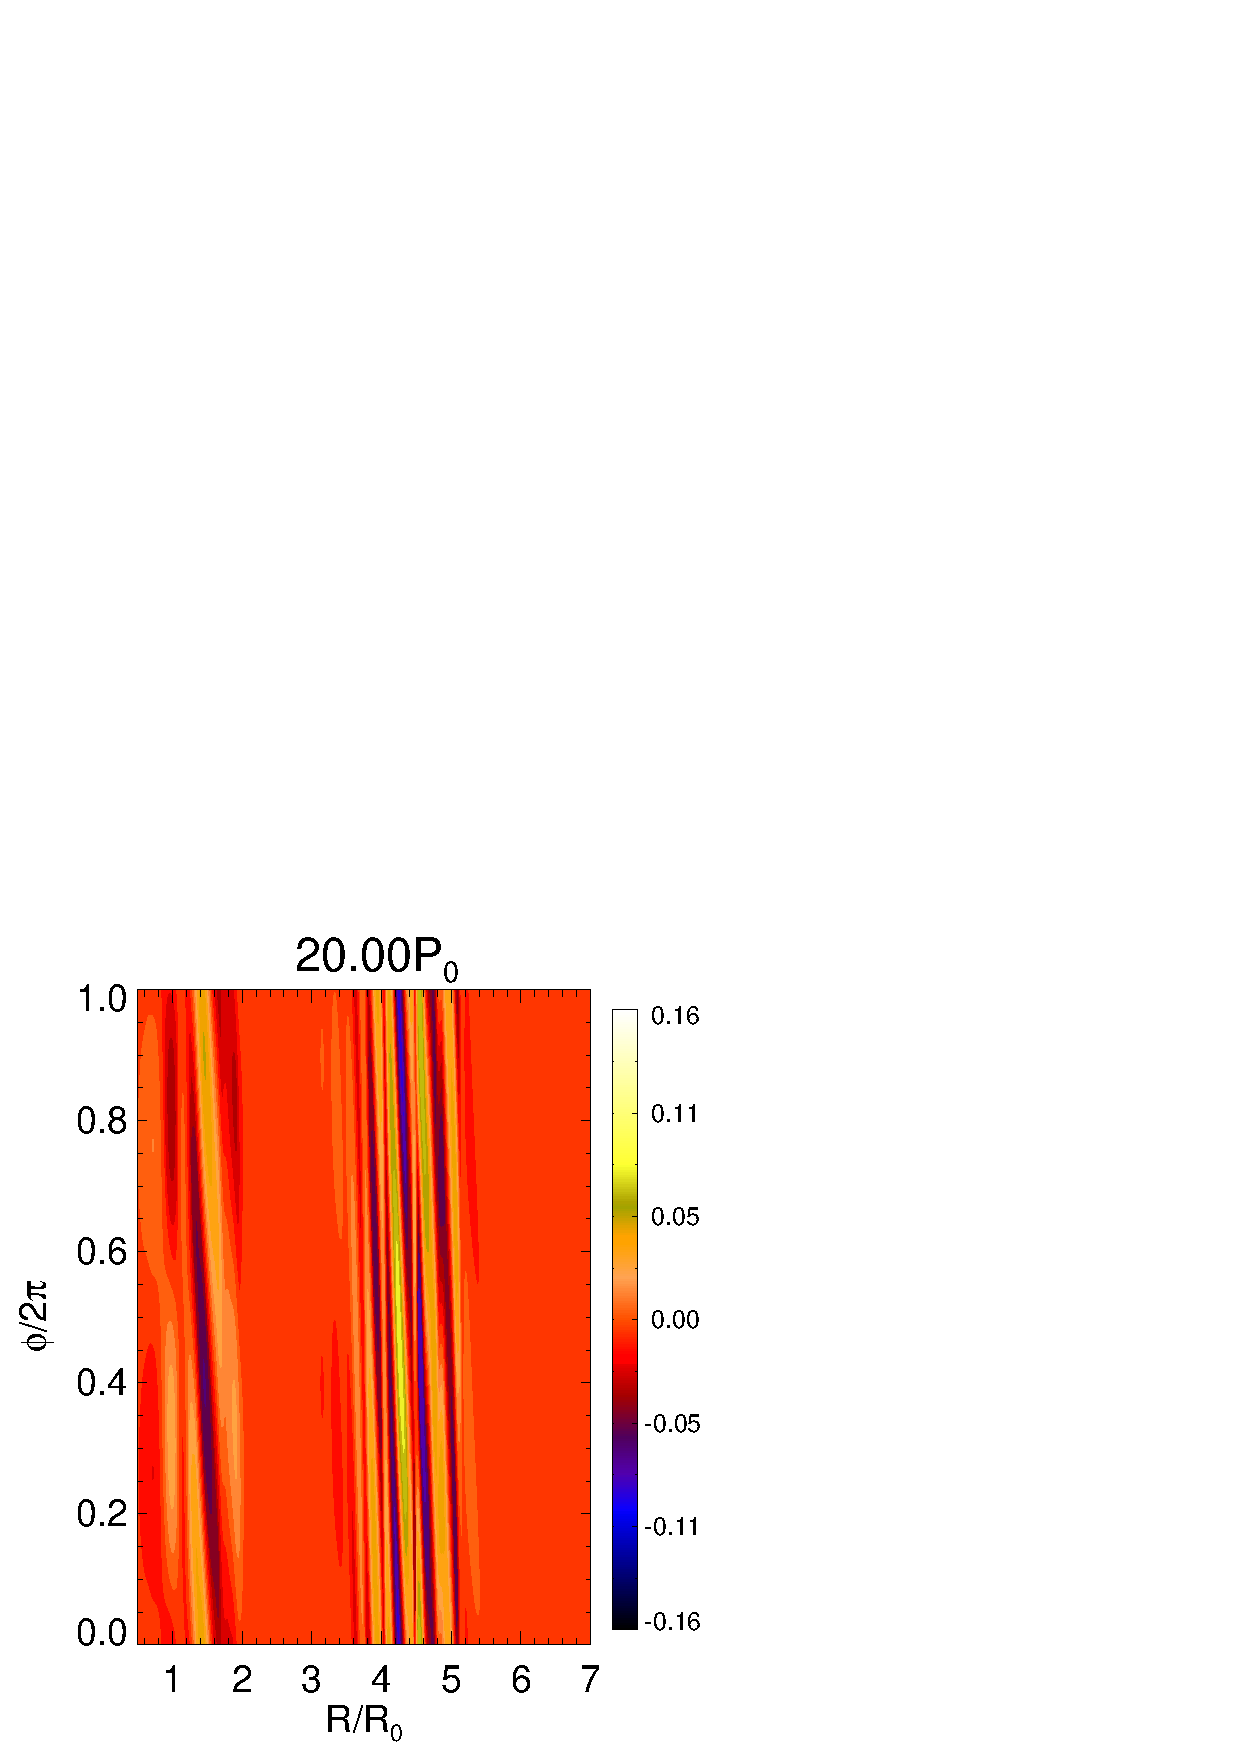
\includegraphics[scale=0.4,clip=true,trim=2.24cm
  0cm 1.73cm 0cm]{figures/polarxy_fargo_ex_200}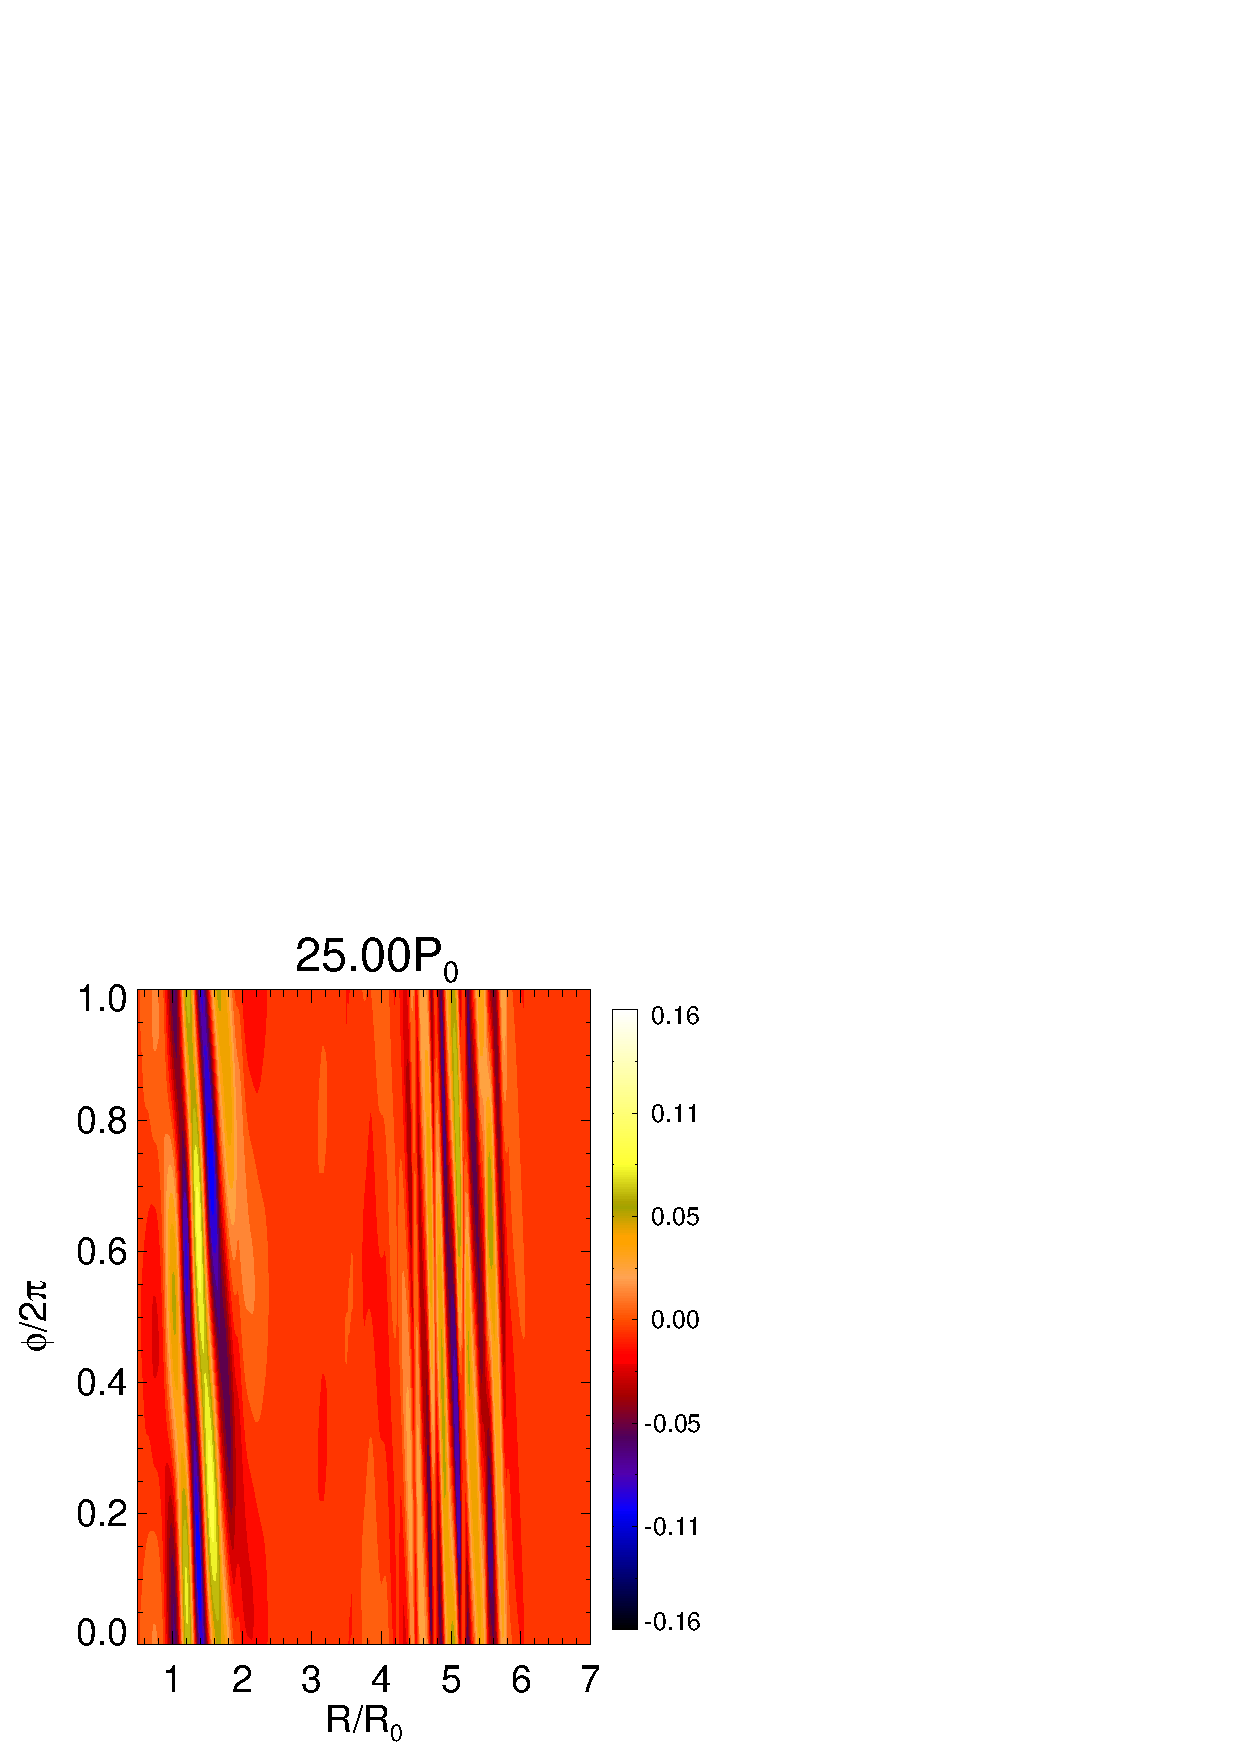
\includegraphics[scale=0.4,clip=true,trim=2.24cm
  0cm 1.73cm 0cm]{figures/polarxy_fargo_ex_250}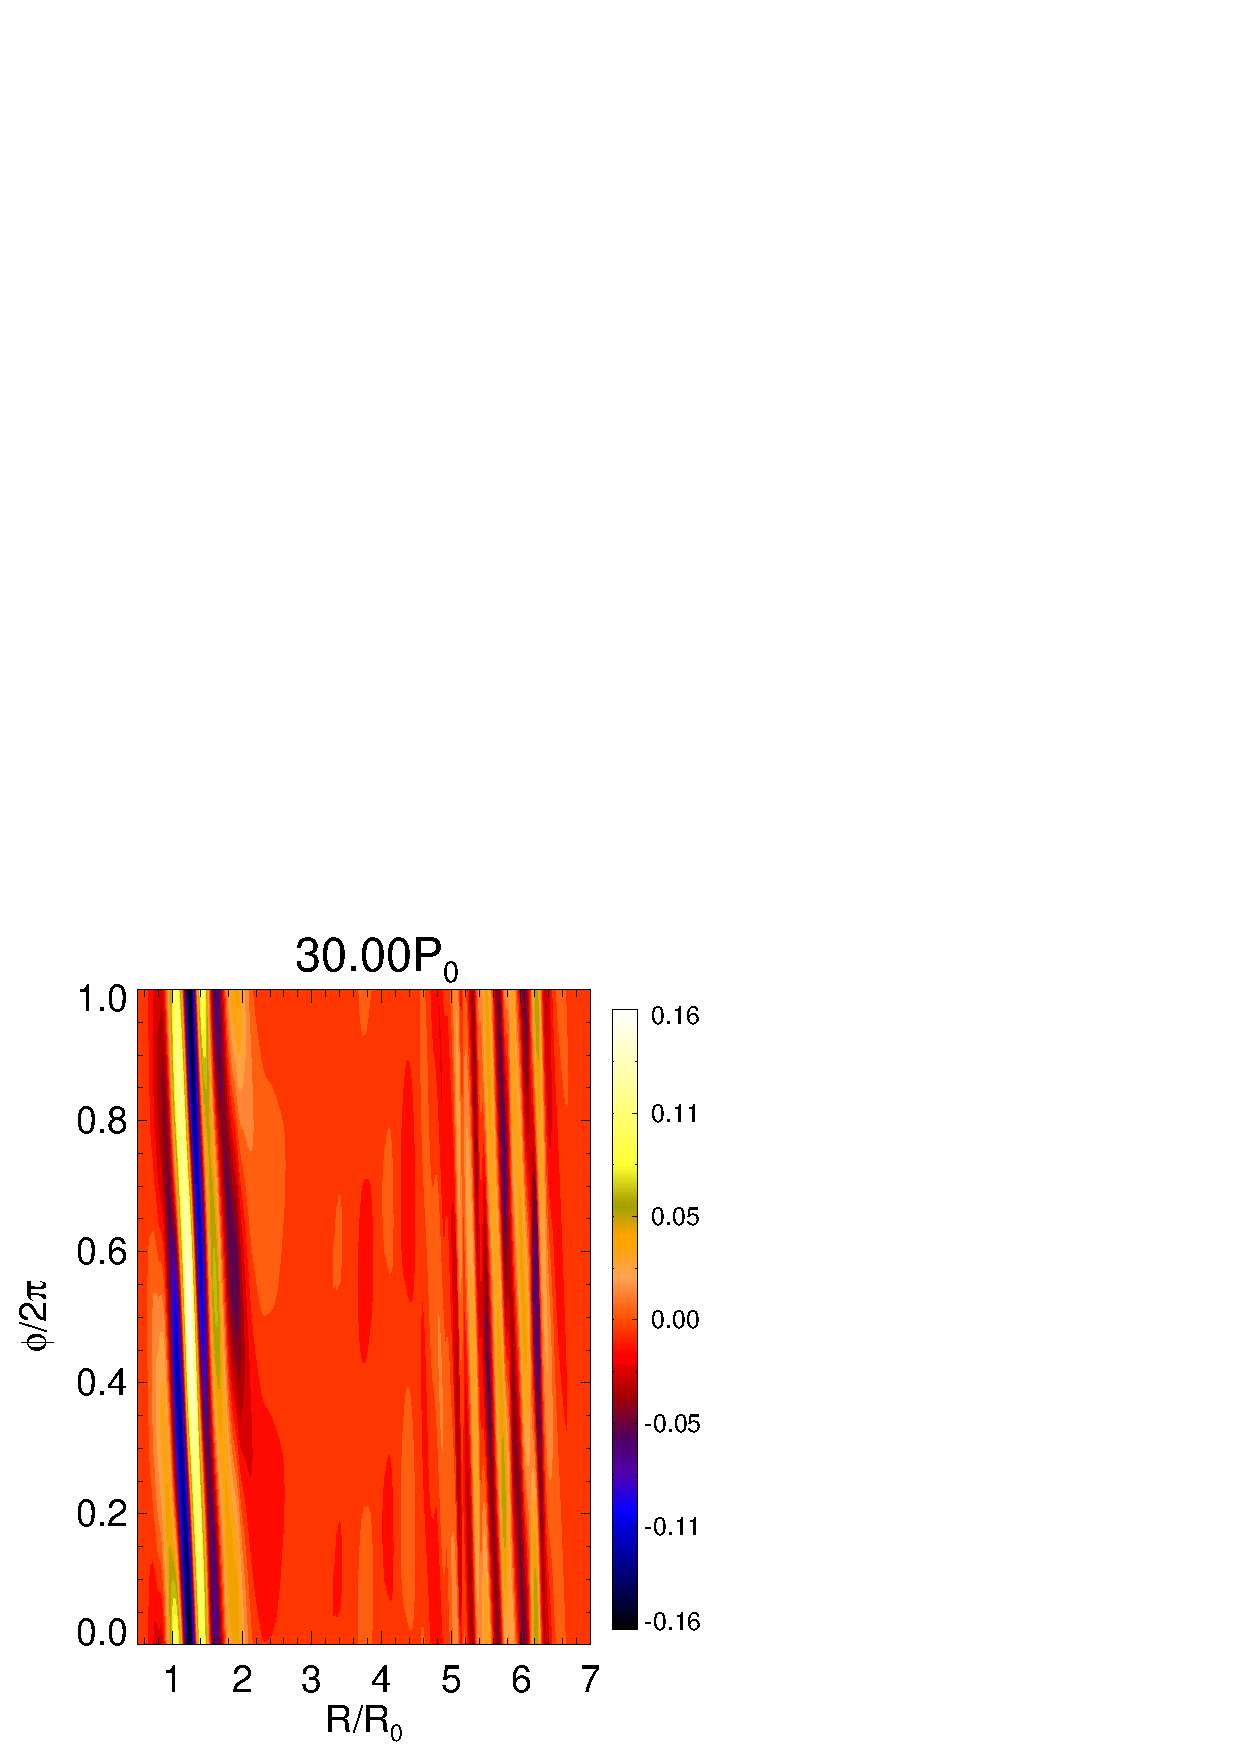
\includegraphics[scale=0.4,clip=true,trim=2.24cm
  0cm 0.0cm 0cm]{figures/polarxy_fargo_ex_300}
  \caption{Evolutoin of the $m=1$ surface density in the FARGO
    simulation with the special $m=1$ initial perturbations
    described in \S\ref{fargo_nonlin}.\label{2d_angmom_ex_evol}} 
\end{figure*}  



\begin{figure}
  % scale=0.41
  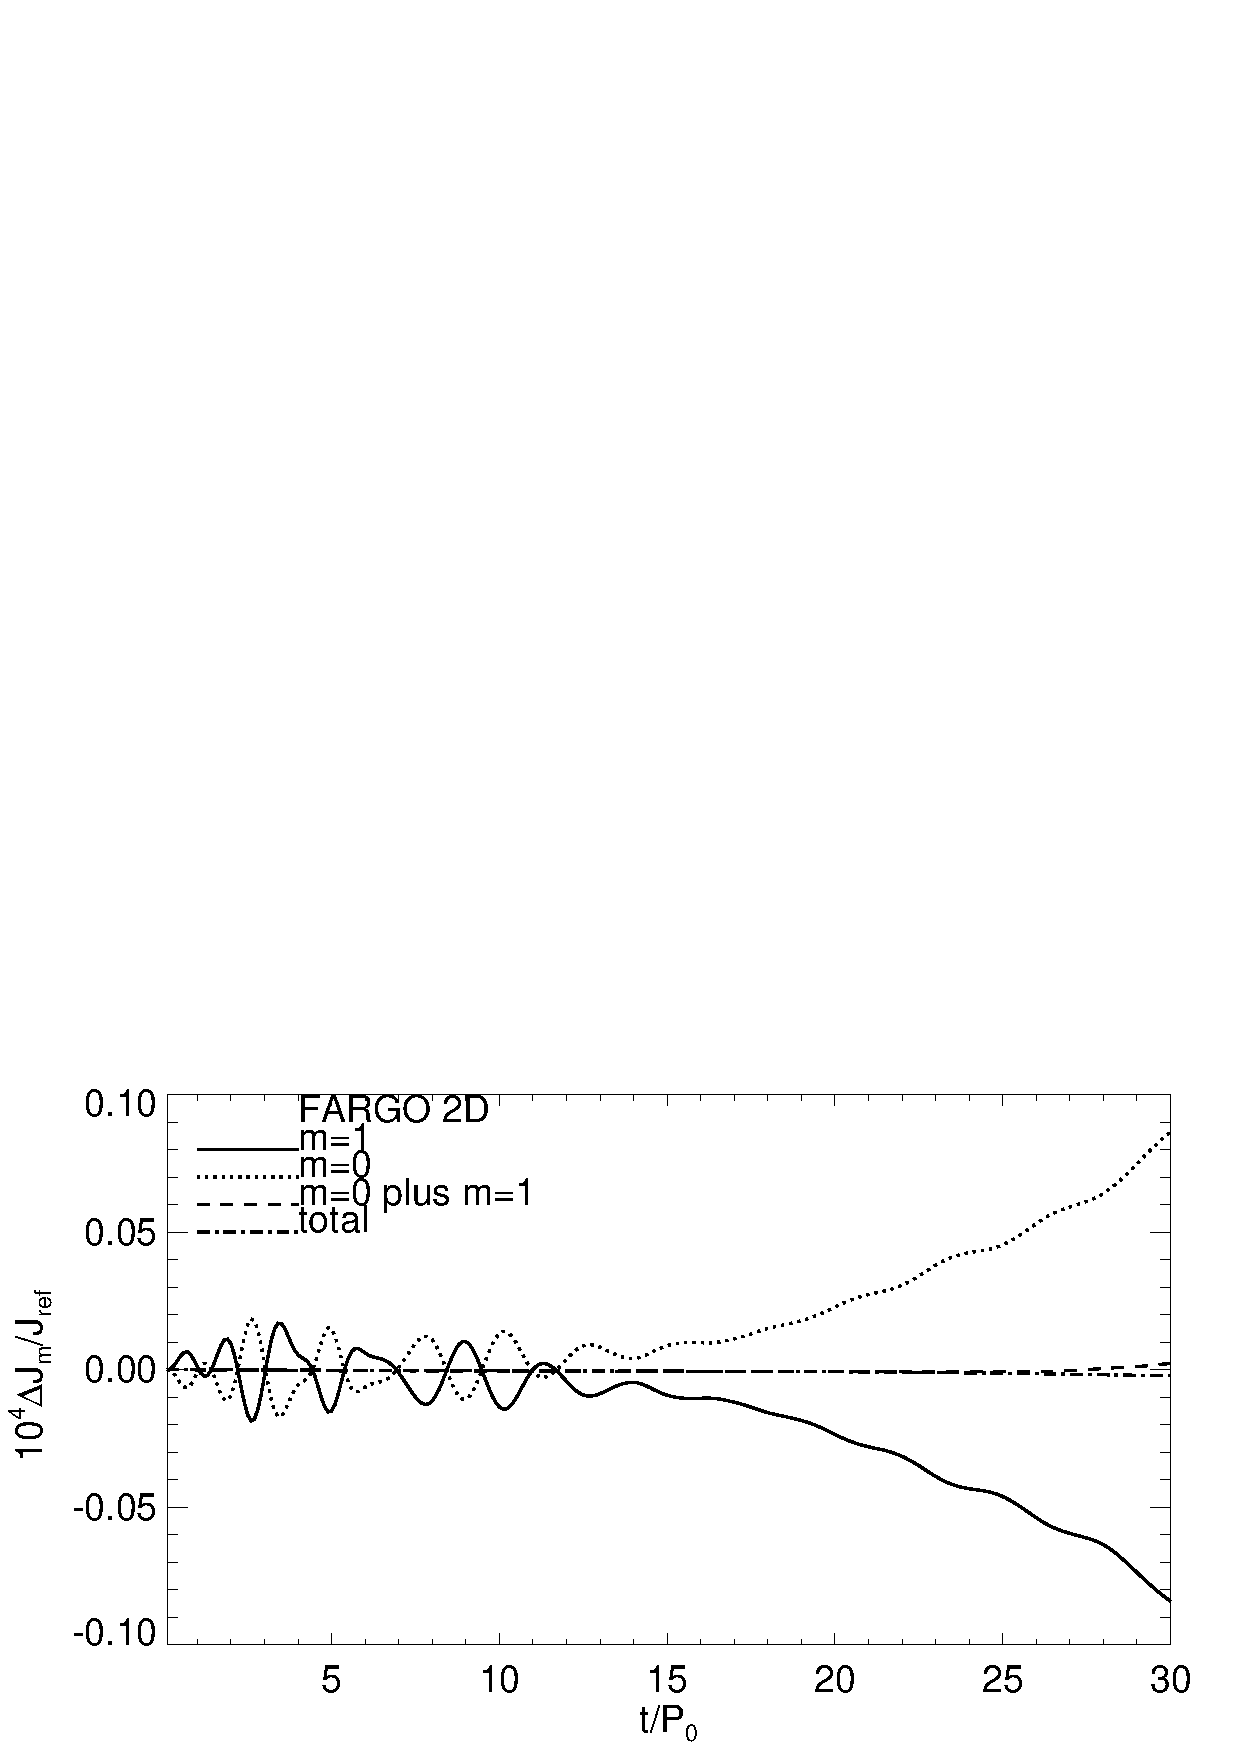
\includegraphics[width=\linewidth]{figures/nonaxi_evol_ang_fargo_ex}
  \caption{Evolution of angular momentum components in the 
    FARGO simulation with the special $m=1$ initial perturbations
    described in \S\ref{fargo_nonlin}. 
    The perturbation
    relative to $t=0$ in 2D is shown in units of the
    initial total angular momentum $J_\mathrm{ref}$.\label{2d_angmom_ex}} 
\end{figure}  